\input{../preamble.tex}
% \bibliographystyle{plain} % Style BST file (bmc-mathphys, vancouver, spbasic).
% \bibliographystyle{unsrt} % Style BST file (bmc-mathphys, vancouver, spbasic).
\bibliography{pubs.bib}      % Bibliography 

\title{Professional Drone, Hybrid Power Pack  - Timebox 8}
\author{Team 2}

\begin{document}
\lstset{language=Matlab,%
  % basicstyle=\color{red},
    inputencoding=latin1,
    breaklines=true,%
    morekeywords={matlab2tikz},
    keywordstyle=\color{blue},%
    morekeywords=[2]{1}, keywordstyle=[2]{\color{black}},
    identifierstyle=\color{black},%
    stringstyle=\color{mylilas},
    commentstyle=\color{mygreen},%
    showstringspaces=false,%without this there will be a symbol in the places where there is a space
    numbers=left,%
    numberstyle={\tiny \color{black}},% size of the numbers
    numbersep=9pt, % this defines how far the numbers are from the text
    emph=[1]{for,end,break},emphstyle=[1]\color{red}, %some words to emphasise
    %emph=[2]{word1,word2}, emphstyle=[2]{style},    
}

\lstset{language=C,%
  % basicstyle=\color{red},
  breaklines=true,%
  morekeywords={matlab2tikz},
  keywordstyle=\color{blue},%
  morekeywords=[2]{1}, keywordstyle=[2]{\color{black}},
  identifierstyle=\color{black},%
  stringstyle=\color{mylilas},
  commentstyle=\color{mygreen},%
  showstringspaces=false,%without this there will be a symbol in the places where there is a space
  % numbers=left,%
  % numberstyle={\tiny \color{black}},% size of the numbers
  % numbersep=9pt, % this defines how far the numbers are from the text
  emph=[1]{for,end,break},emphstyle=[1]\color{red}, %some words to emphasise
  % emph=[2]{word1,word2}, emphstyle=[2]{style},    
}
% \lstdefinestyle{customc}{
%   belowcaptionskip=1\baselineskip,
%   breaklines=true,
%   frame=L,
%   xleftmargin=\parindent,
%   language=C,
%   showstringspaces=false,
%   basicstyle=\footnotesize\ttfamily,
%   keywordstyle=\bfseries\color{green!40!black},
%   commentstyle=\itshape\color{purple!40!black},
%   identifierstyle=\color{blue},
%   stringstyle=\color{orange},
% }

% \lstdefinestyle{customasm}{
%   belowcaptionskip=1\baselineskip,
%   frame=L,
%   xleftmargin=\parindent,
%   language=[x86masm]Assembler,
%   basicstyle=\footnotesize\ttfamily,
%   commentstyle=\itshape\color{purple!40!black},
% }

% \lstset{escapechar=@,style=customc}

\newcounter{udrboks}[section]\setcounter{udrboks}{0}
\renewcommand{\theudrboks}{\arabic{section}.\arabic{udrboks}}
\renewcommand{\theudrboks}{\arabic{udrboks}}
\newenvironment{udrboks}[2][]{%
  \refstepcounter{udrboks}%
  \ifstrempty{#1}%
  {\mdfsetup{%
      frametitle={%
        \tikz[baseline=(current bounding box.east),outer sep=0pt]
        \node[anchor=east,rectangle,fill=blue!20]
        {\strut Udregninger~\theudrboks};}}
  }%
  {\mdfsetup{%
      frametitle={%
        \tikz[baseline=(current bounding box.east),outer sep=0pt]
        \node[anchor=east,rectangle,fill=blue!20]
        {\strut Udregninger ~\theudrboks:~#1};}}%
  }%
  \mdfsetup{innertopmargin=10pt,linecolor=blue!20,%
    linewidth=2pt,topline=true,%
    frametitleaboveskip=\dimexpr-\ht\strutbox\relax
  }
  \begin{mdframed}[]\relax%
    \label{#2}}{\end{mdframed}}


\newcounter{formelboks}[section]\setcounter{formelboks}{0}
\renewcommand{\theformelboks}{\arabic{section}.\arabic{formelboks}}
\renewcommand{\theformelboks}{\arabic{formelboks}}
\newenvironment{formelboks}[2][]{%
  \refstepcounter{formelboks}%
  \ifstrempty{#1}%
  {\mdfsetup{%
      frametitle={%
        \tikz[baseline=(current bounding box.east),outer sep=0pt]
        \node[anchor=east,rectangle,fill=blue!20]
        {\strut Formler~\theformelboks};}}
  }%
  {\mdfsetup{%
      frametitle={%
        \tikz[baseline=(current bounding box.east),outer sep=0pt]
        \node[anchor=east,rectangle,fill=blue!20]
        {\strut Formler ~\theformelboks:~#1};}}%
  }%
  \mdfsetup{innertopmargin=10pt,linecolor=blue!20,%
    linewidth=2pt,topline=true,%
    frametitleaboveskip=\dimexpr-\ht\strutbox\relax
  }
  \begin{mdframed}[]\relax%
    \label{#2}}{\end{mdframed}}

\newcounter{konstboks}[section]\setcounter{konstboks}{0}
\renewcommand{\thekonstboks}{\arabic{section}.\arabic{konstboks}}
\newenvironment{konstboks}[2][]{%
  \refstepcounter{konstboks}%
  \ifstrempty{#1}%
  {\mdfsetup{%
      frametitle={%
        \tikz[baseline=(current bounding box.east),outer sep=0pt]
        \node[anchor=east,rectangle,fill=green!20]
        {\strut Konstanter~\thekonstboks};}}
  }%
  {\mdfsetup{%
      frametitle={%
        \tikz[baseline=(current bounding box.east),outer sep=0pt]
        \node[anchor=east,rectangle,fill=green!20]
        {\strut Konstanter~\thekonstboks:~#1};}}%
  }%
  \mdfsetup{innertopmargin=10pt,linecolor=green!20,%
    linewidth=2pt,topline=true,%
    frametitleaboveskip=\dimexpr-\ht\strutbox\relax
  }
  \begin{mdframed}[]\relax%
    \label{#2}}{\end{mdframed}}
\pgfplotstableread[row sep=\\,col sep=&]{
  ide & stemmer  \\
  Paraply & 9  \\
  Fjernbetjening & 7  \\
  iAdapt & 2 \\
}\mydata
% \setcounter{secnumdepth}{1}
\maketitle
\thispagestyle{empty}

\textbf{Deltagere:}
\begin{figure}[h]
  \centering
  % BEGIN RECEIVE ORGTBL delt
  \begin{tabular}{|p{5cm}p{10cm}|}
    \hline
    &\\
    Stud. nr: 201602094 & Navn: Søren Holm Korsgaard \\
    \hline
    &\\
    Stud.nr.: 201607563 & Navn: Jacob Gustafsson \\
    \hline
    &\\
    % Stud.nr.: 201704859 & Navn: Jonas Buus \\
    % \hline
    % &\\
    Stud.nr.: 20084327 & Navn: Simon Rasmussen \\
    \hline
    &\\
    Stud.nr.: 201704483 & Navn: Thomas Dueholm Jensen \\
    \hline
  \end{tabular}
  % END RECEIVE ORGTBL delt

\end{figure}
\vspace{-5mm}
% \clearpage
\setcounter{tocdepth}{2}
\tableofcontents
\thispagestyle{empty}
\newpage
% \pagenumbering{arabic}
\setcounter{page}{1}

% \section{Introduktion}
% \label{sec:introduktion}

\section{Strategy and planning (Jacob)}
\label{sec:strategy-planning}

I forbindelse med Timebox nr. 8 er arbejdet fortsat med spændingsregulator, aktiv ensretter og PID-regulering. Gruppen er stadig betinget af, at vi ikke har fået klarhed for Jonas’ videre deltagelse. I forbindelse hermed er Development Plan blevet opdateret, og gjort mere overskuelig, da tidligere uger er blevet fjernet. 
Development plan kan ses herunder. 

\begin{figure}[h]
  \centering
  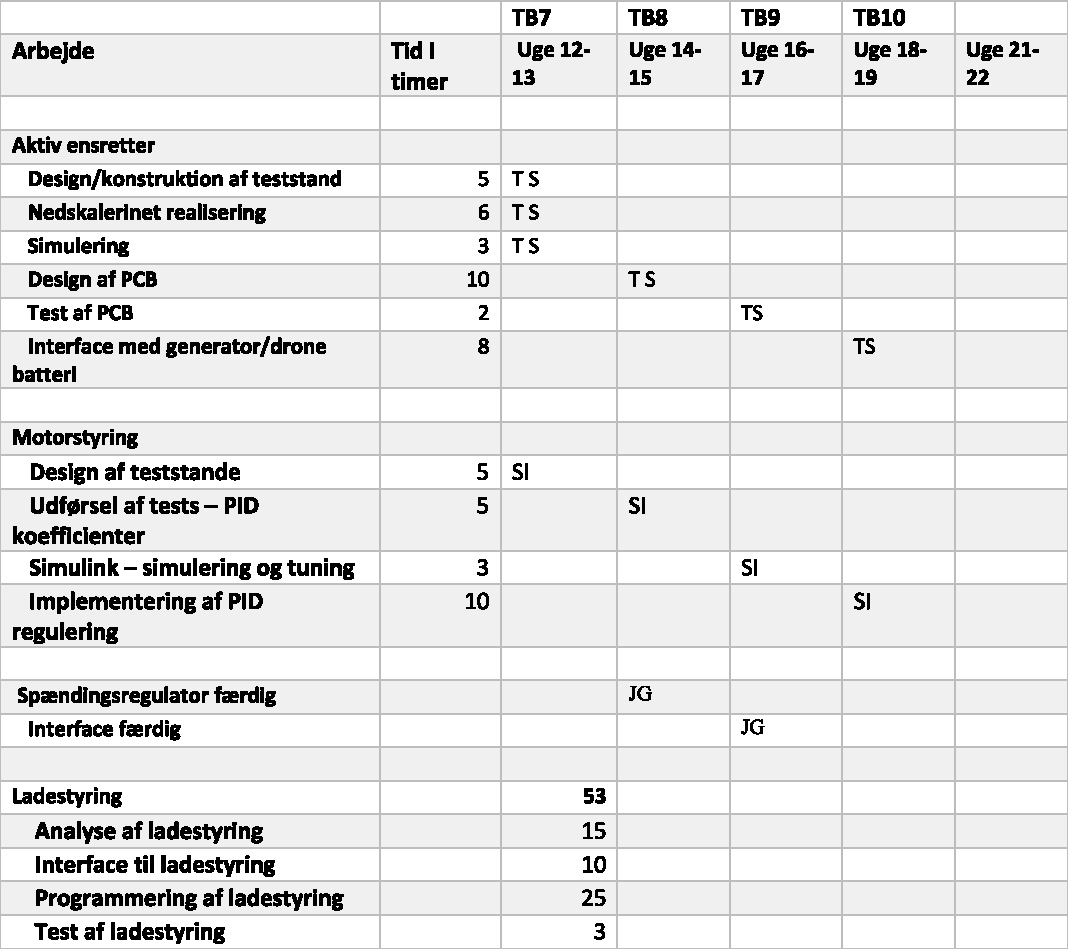
\includegraphics[width=0.6\textwidth]{plan.pdf}
  \caption{Development plan}
  \label{fig:plan}
\end{figure}

Som det ses af planen er der stadig dele af projektet, som ikke er færdiggjort, med hvilket arbejdet fortsætter i næste timebox.

\subsection{Spændingsregulator}
\label{sec:spandingsregulator}
Jf. Development Planen skal spændingsregulatoren være færdig i denne uge, hvilket også er tilfældet. Derfor deployes den færdige spændingsregulator i timebox 8. 

\subsection{Aktiv ensretter}
\label{sec:aktiv-ensretter}
Den aktive ensretter er også færdig og loddet på print. Denne deployes i denne timebox. 

\subsection{Motorstyring}
\label{sec:motorstyring}
Til motorstyringen er der i denne timebox målinger analyseret og der er udledt overføringsfunktion.
\clearpage
\section{Spændingsregulator (Jacob)}
\label{sec:spandingsregulator-1}

Spændingsregulatoren gøres færdig i denne timebox. Heraf følger endeligt valg af spændingsregulatoren, samt opsætning af PCB og endelig test af den færdige løsning.

\subsection{Analysen}
\label{sec:analysen}

Spændingsregulatoren skal levere strøm til vores logiske kredsløb.

\subsubsection{Kravsspecifikation}
\label{sec:kravsspecifikation}

\textbf{Uniquituos}
\begin{itemize}
\item Skal regulere en spænding fra 22 V til 5 V 
\item Skal kunne håndtere strømme på 1 A 
\item Driftssikker, også ved påvirkning af varme - 2 P
\item Skal være den billigste, brugbare løsning - 2 P
\item Minimal ripple på output - 1 P
\item Minimal størrelse og vægt - 1 P
\item Skal være vejrbestandig 
\end{itemize}

For at kunne bestemme, hvilken spændingsregulator der bruges, er kravene delt op. De 2 øverste skal være opfyldt, før at systemet kan komme i betragtning. De 3 mellemstående tildeles point efter vigtigheden, og det nederste krav klares udenom systemet i begge tilfælde.

\subsection{Interface - Analyse og Design }
\label{sec:interface-analyse-og}

Spændingsregulatoren bliver et system placeret mellem batteripakken og de logiske kredsløb samt som forsyningsspænding til visse IC-kredse på ensretteren samt tændspolen.

\begin{figure}[h]
  \centering
  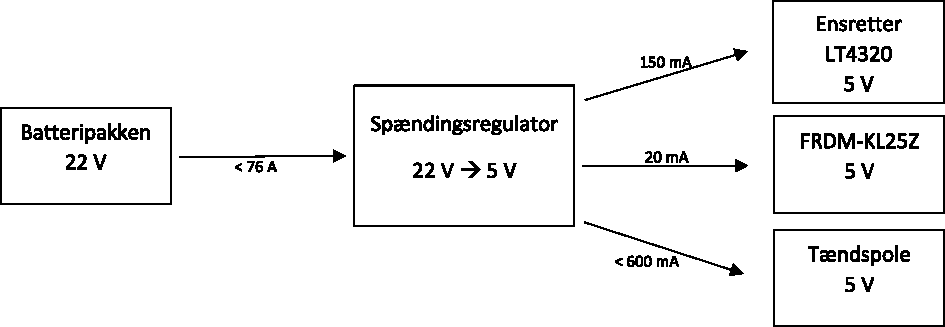
\includegraphics[width=0.6\textwidth]{jfig1.pdf}
  \caption{Diagram over hvilken sammenhæng spændingsregulatoren skal fungere i.}
  \label{fig:dia1}
\end{figure}

Herover vises et diagram over, hvilken sammenhæng spændingsregulatoren skal fungere i. Påtrykt er også de strømme, som der bliver trukket fra spændingsregulatoren. Da regulatoren er forbundet med batteripakken, har den op til 76 A til rådighed. De maksimale strømme summeret, giver et strømbehov på 769 mA RMS. Derfor har vi valgt, at spændingsregulatoren skal kunne håndtere 1 A RMS. Alle 3 systemer, som kobles op til spændingsregulatoren, skal bruge en forsyning på mellem 3,3 V og 5 V. 
For at sikre en minimal resistans til og fra systemet bruges 1 mm2 ledere til og fra systemet. Af nomogrammet fra baadteknik.dk aflæses, at 20 W kan distribueres op til cirka 4 meter med en leder af denne tykkelse. Da vores afstande er meget mindre, er vi sikre på at denne ledningstykkelse er tilstrækkelig. 


\subsection{Test af systemerne}
\label{sec:test-af-systemerne}

\subsubsection{LM-317}
\label{sec:lm-317}
\textbf{Design og simulering}\newline
Systemet der baseres på en LM-317T er vist herunder. Her ses også resultatet af simuleringen.

\begin{figure}[h]
  \centering
  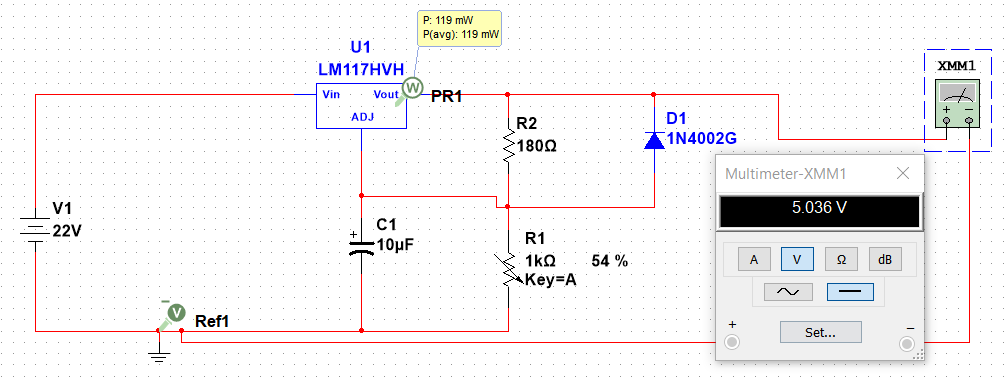
\includegraphics[width=0.7\textwidth]{bil1.png}
  \caption{Systemet der baseres på en LM-317T}
  \label{fig:bil1}
\end{figure}

Prisen for systemet her er listet nedenfor. Komponenter der allerede findes i EL-LAB er listet til 0 kr.
\begin{table}[h]
  \centering
% BEGIN RECEIVE ORGTBL tabel1
\begin{tabular}{ll}
\hline
Komponent & Pris i DKR \\
\hline
LM317-T (erstatter LM117-HVH) & 0,- \\
\hline
Kondensator & 0,- \\
\hline
Variabel modstand & 0,- \\
\hline
Modstand & 0,- \\
\hline
Diode & 0,- \\
\hline
IALT & 0,- \\
\hline
\end{tabular}
% END RECEIVE ORGTBL tabel1
  \caption{Kompenenter}
  \label{tab:komp}
\end{table}
\begin{comment}
#+ORGTBL: SEND tabel1 orgtbl-to-latex :splice nil :skip 0
|-------------------------------+------------|
| Komponent                     | Pris i DKR |
|-------------------------------+------------|
| LM317-T (erstatter LM117-HVH) | 0,-        |
|-------------------------------+------------|
| Kondensator                   | 0,-        |
|-------------------------------+------------|
| Variabel modstand             | 0,-        |
|-------------------------------+------------|
| Modstand                      | 0,-        |
|-------------------------------+------------|
| Diode                         | 0,-        |
|-------------------------------+------------|
| IALT                          | 0,-        |
|-------------------------------+------------|
\end{comment}
\clearpage
\textbf{Realisering}\newline
Realiseringen af systemet sker i første omgang på breadboard, hvor det er nemt at lave ændringer til systemet. Som det ses af billedet, er størrelsen meget beskeden. Komponenterne vil endda kunne samles yderligere, når printet skal designes, ligesom klemmen til multimeteret kan udelades.
På det andet billede ses systemet under påvirkning af varme. Varmen blev primært tilført LM317-T, men også modstandene blev udsat for varme.

\begin{figure}[h]
  \centering
  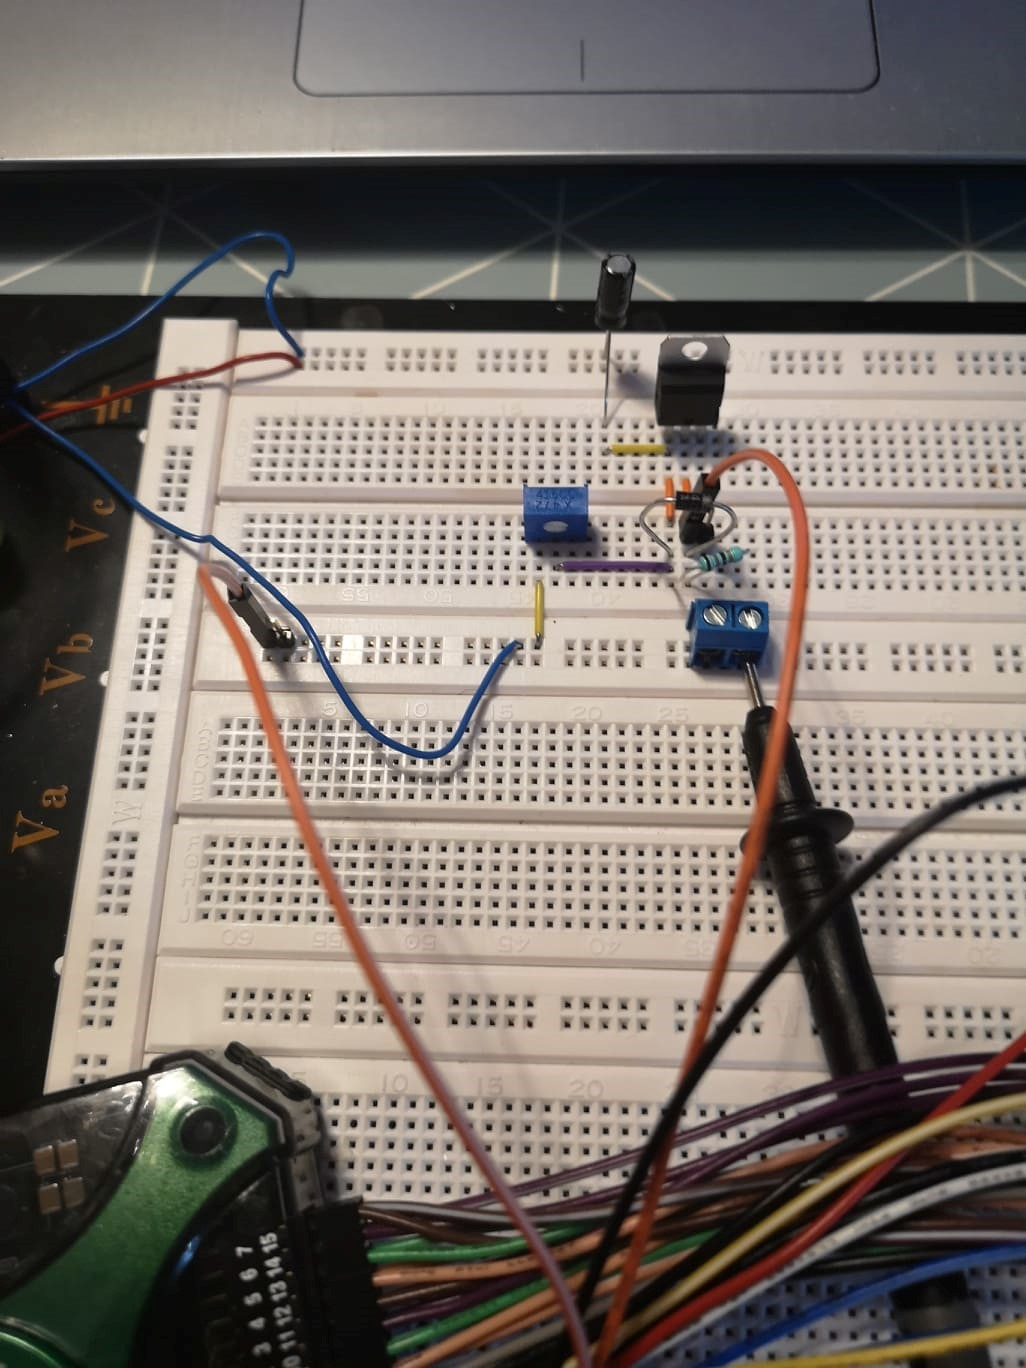
\includegraphics[width=0.3\textwidth]{bil2.jpg}
  \caption{Realisering af systemet}
  \label{fig:bil2}
\end{figure}

% \begin{figure}[h]
%   \centering
%   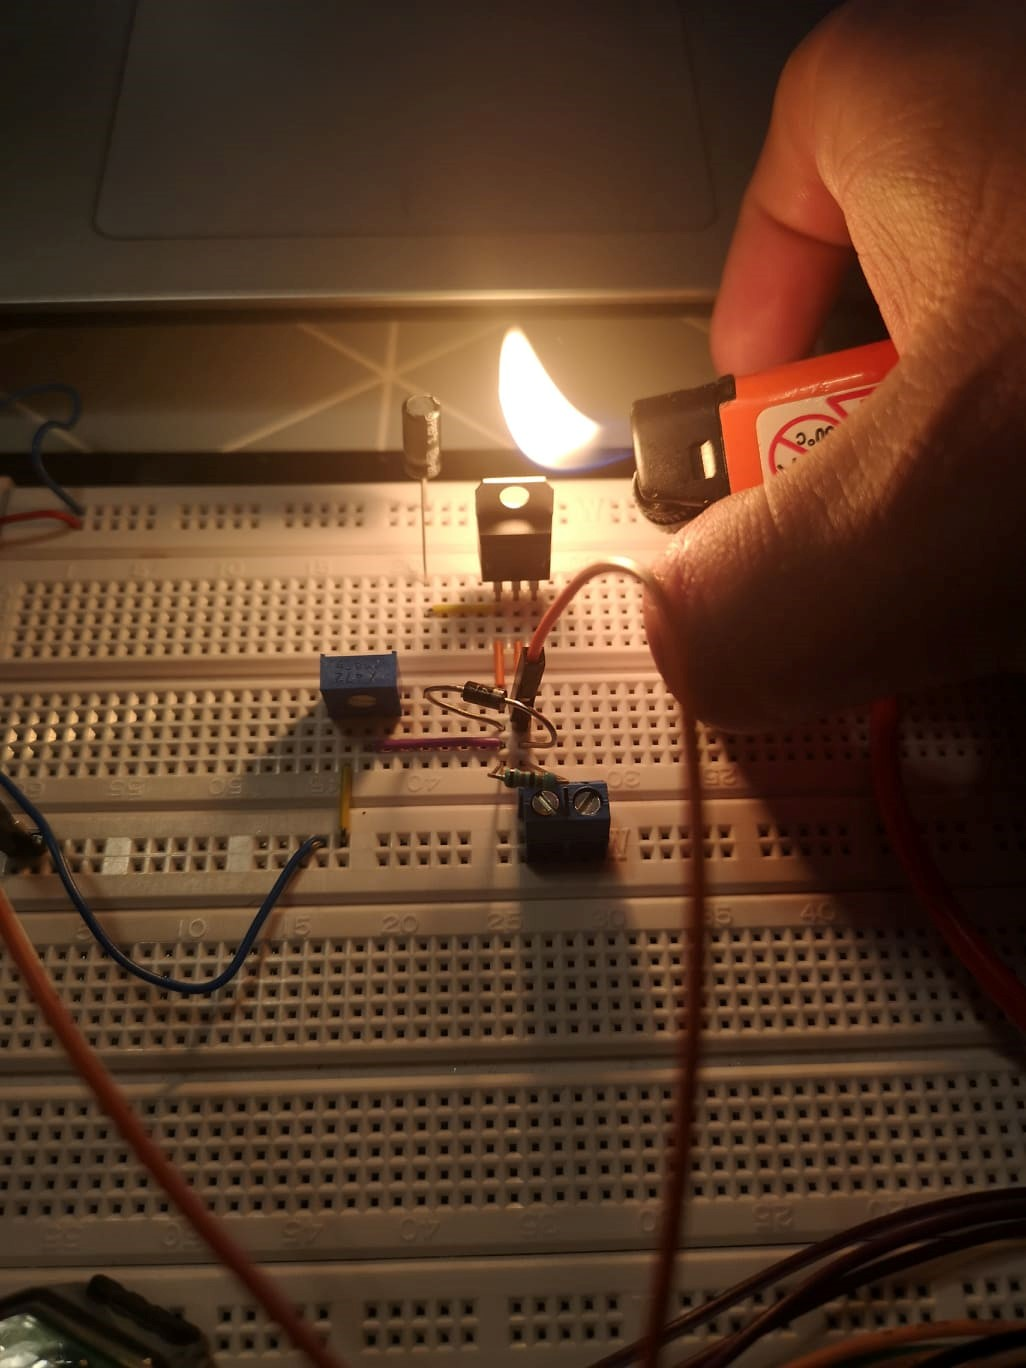
\includegraphics[width=\textwidth]{bil3.jpg}
%   \caption{Systemet under påvirkning af varme}
%   \label{fig:bil3}
% \end{figure}

\textbf{Testresultater}\newline
Hernæst følger resultaterne fra testen af LM317-T .

Det første billede viser outputtet under almindelige forhold.
\begin{figure}[h]
  \centering
  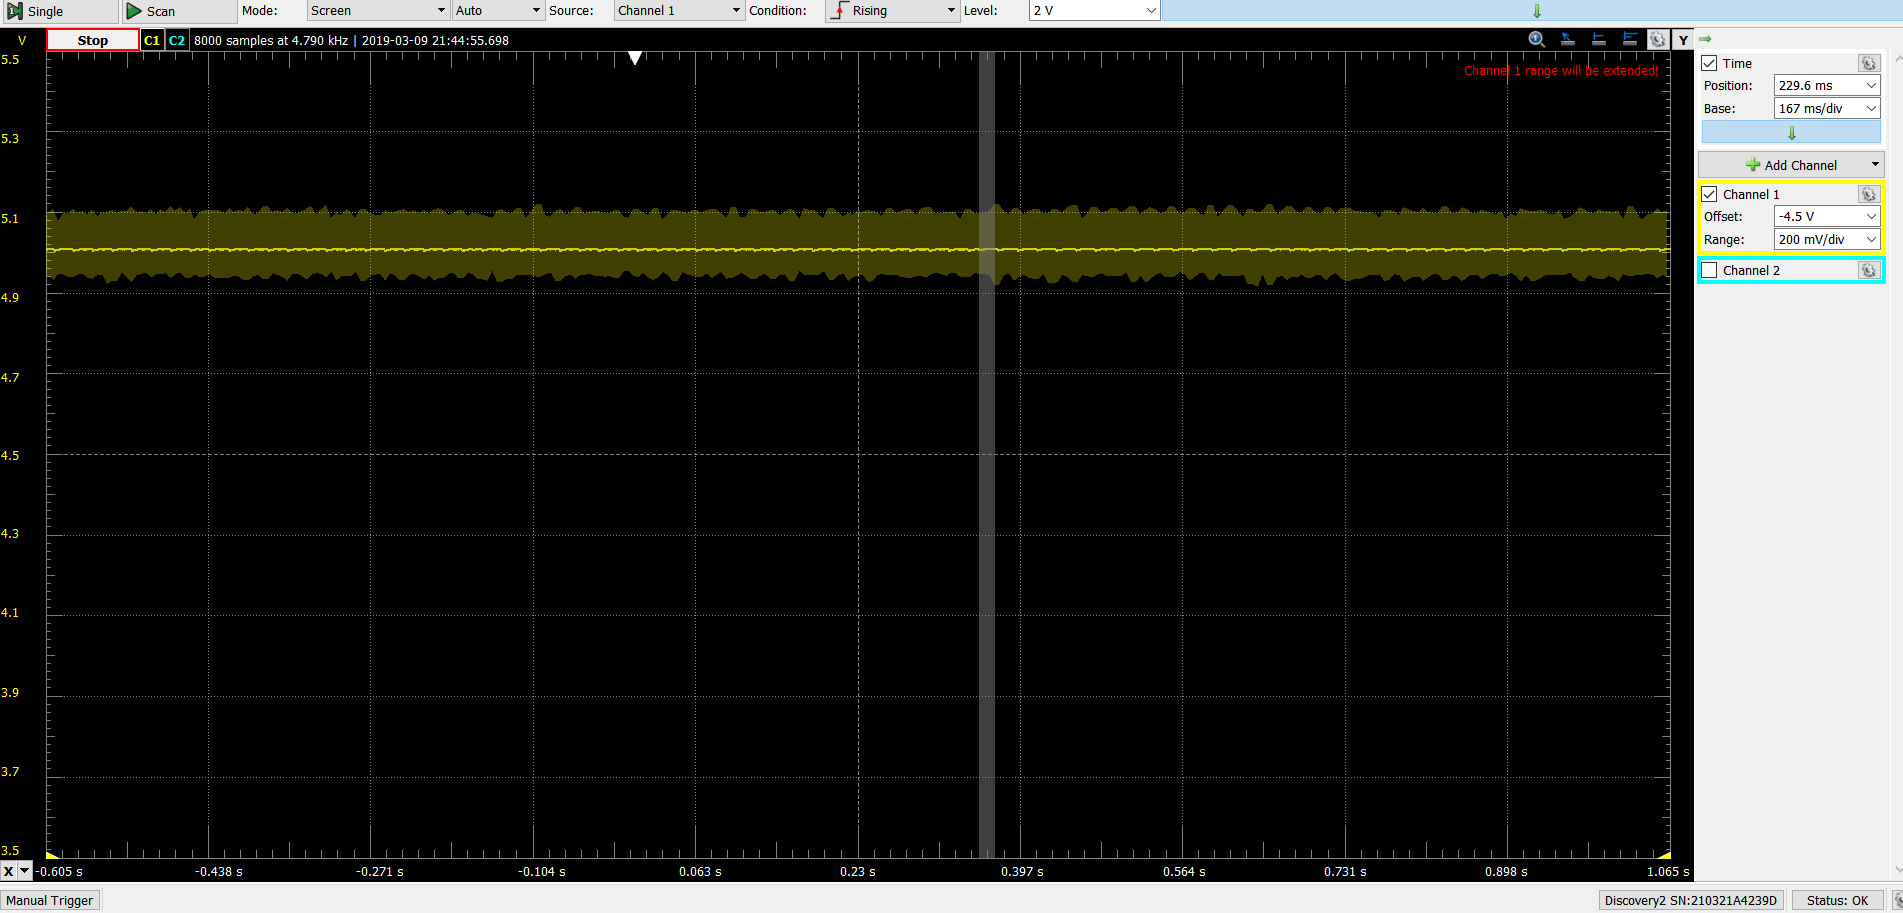
\includegraphics[width=0.3\textwidth]{bil4.png}
  \caption{}
  \label{fig:bil4}
\end{figure}


% \begin{figure}
% \centering
% \begin{subfigure}{.5\textwidth}
%   \centering
%   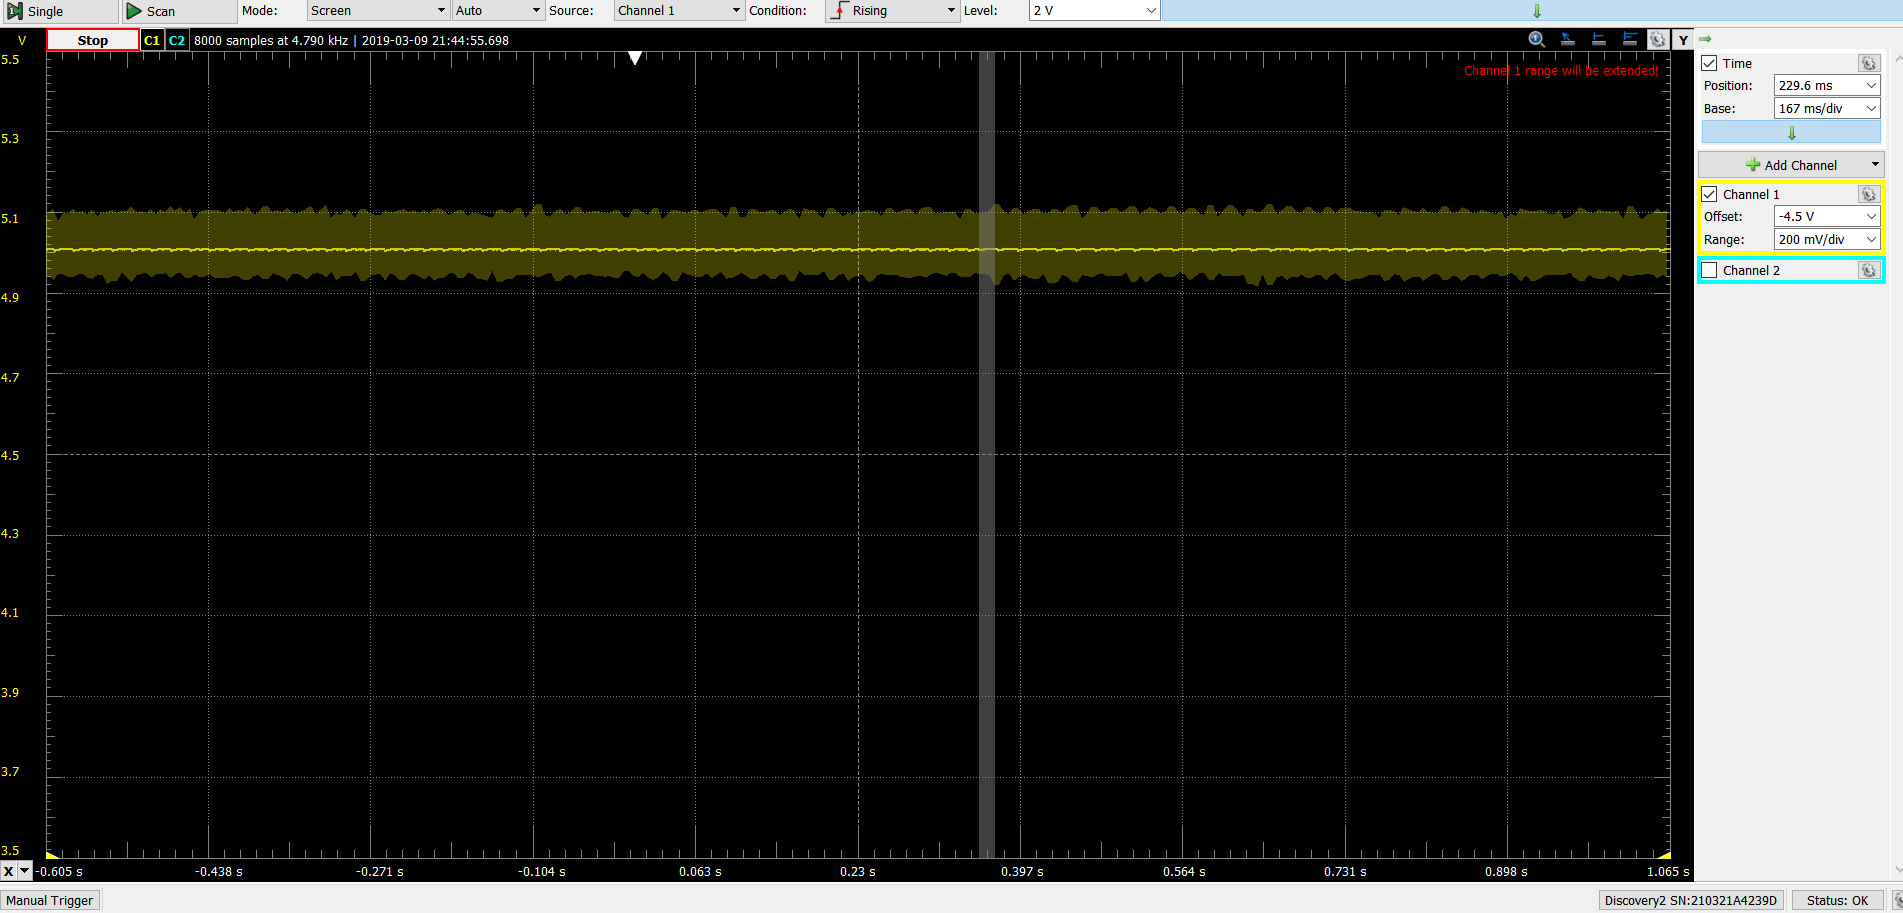
\includegraphics[width=1\linewidth]{bil4.png}
%   % \caption{A subfigure}
%   \label{fig:sub1}
% \end{subfigure}%
% \begin{subfigure}{.5\textwidth}
%   \centering
%   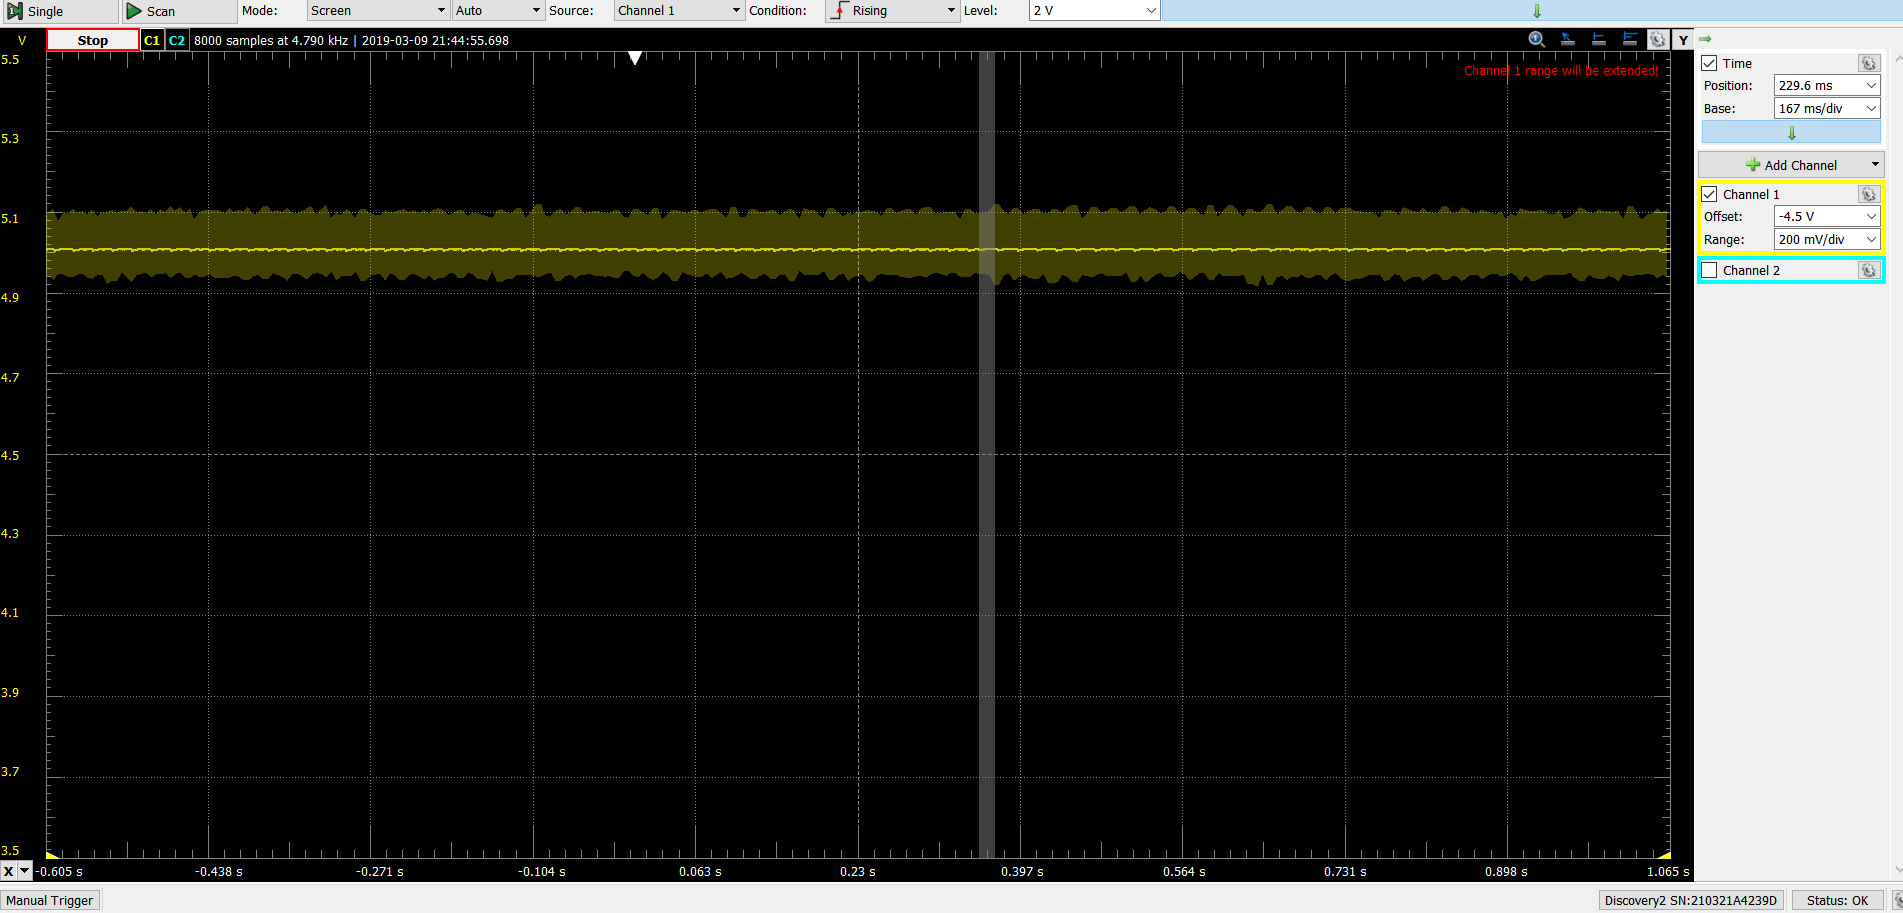
\includegraphics[width=1\linewidth]{bil5.png}
%   % \caption{A subfigure}
%   \label{fig:sub2}
% \end{subfigure}
% % \caption{A figure with two subfigures}
% \label{fig:test}
% \end{figure}
\clearpage
Som det tydeligt ses af det zoomede billede, ligger vores output på de ønskede 5 V. Ved at påsætte en målemodstand på outputtet blev der målt en strøm på 1,07 A, hvilket er tilstrækkeligt i vores tilfælde. Ifølge datasheetet kan LM317-T håndtere op til 1,5 A.

\begin{figure}[h]
  \centering
  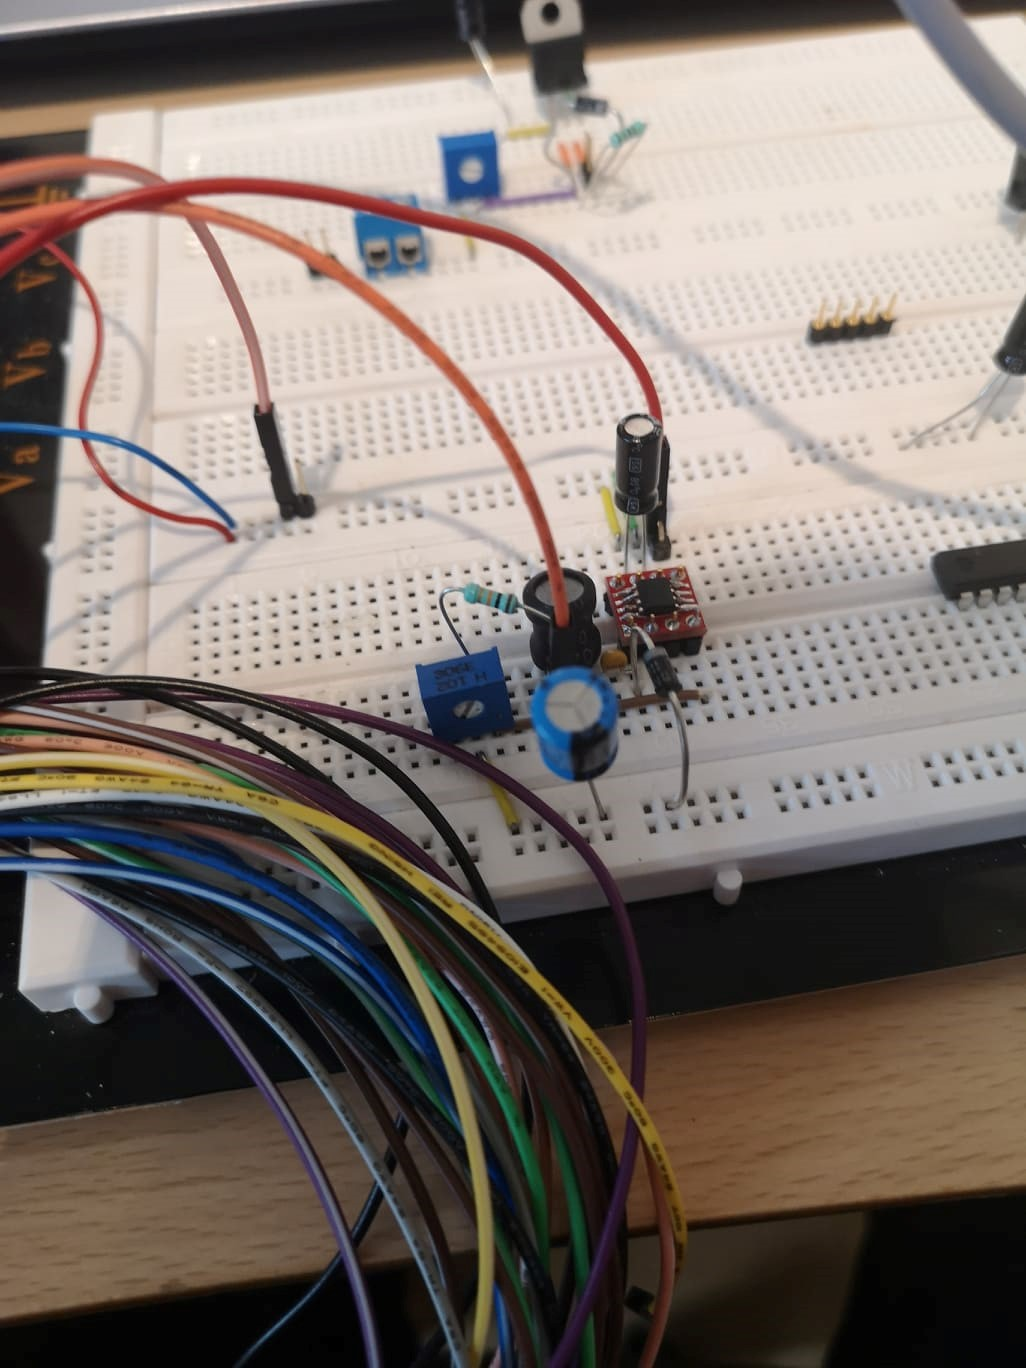
\includegraphics[width=0.3\textwidth]{bil6.jpg}
  \caption{}
  \label{fig:bil6}
\end{figure}

Efter at udsætte systemet for varme, ændrede outputtet sig en smule. Det største udsving ses, når det er LM317-T der udsættes for lighteren. Her ses outputtet efter 30 sekunders påvirkning. Vi kan altså konkludere, at spændingen ikke engang falder 0,1 V.
Efter testen måles modstanden på den variable modstand til 538 ohm.

\subsubsection{TPS5410}
\label{sec:tps5410}

\textbf{Design og simulering}\newline
Systemet der baseres på en TPS5410 BUCK-converter ses herunder. Designet er udarbejdet med onlineværktøjet WEBENCH fra Texas Instruments. 

\begin{figure}[h]
  \centering
  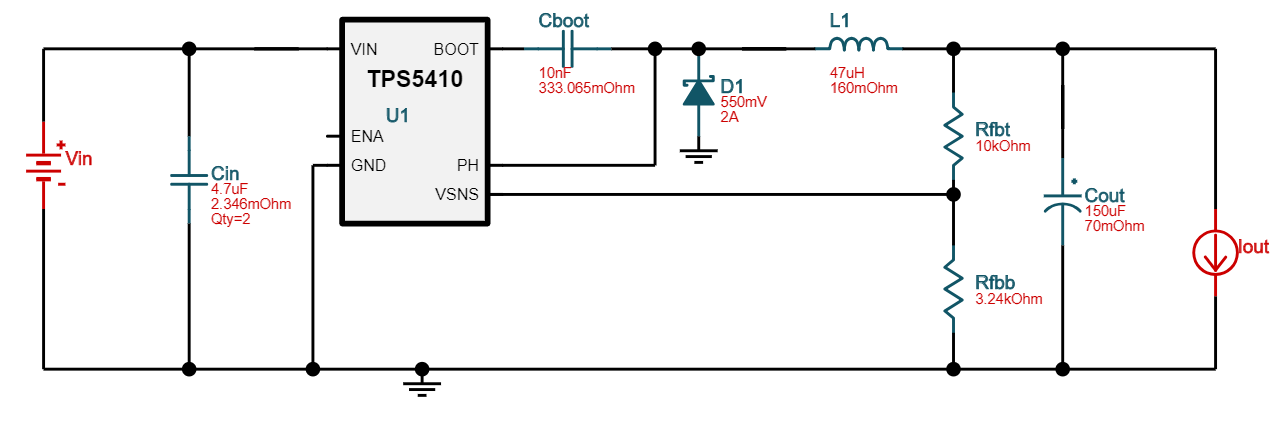
\includegraphics[width=0.5\textwidth]{dia2.png}
  \caption{}
  \label{fig:bil6}
\end{figure}

Da TPS5410 ikke findes i Multisim, har det ikke været muligt at lave en simulering af systemet.


Prisen for systemet er listet nedenfor. Ligesom i ovenstående tilfælde vil komponenter der allerede findes i EL-LAB være angivet til DKR 0,-.

\clearpage
\begin{table}[h]
  \centering
% BEGIN RECEIVE ORGTBL tabel2
\begin{tabular}{ll}
\hline
Komponent & Pris i DKR \\
\hline
TPS5410 & 21,36 \\
\hline
Kondensator & 0,- \\
\hline
Modstande & 0,- \\
\hline
Diode & 30,28 (minimumskøb = 10 stk.) \\
\hline
Spole & 42,16 \\
\hline
Adapter (SMD$\rightarrow$  DIL8) & 21,- \\
\hline
IALT & 0,- \\
\hline
\end{tabular}
% END RECEIVE ORGTBL tabel2
  \caption{Kompenenter}
  \label{tab:komp2}
\end{table}
\begin{comment}
#+ORGTBL: SEND tabel2 orgtbl-to-latex :splice nil :skip 0
|---------------------+-------------------------------|
| Komponent           | Pris i DKR                    |
|---------------------+-------------------------------|
| TPS5410             | 21,36                         |
|---------------------+-------------------------------|
| Kondensator         | 0,-                           |
|---------------------+-------------------------------|
| Modstande           | 0,-                           |
|---------------------+-------------------------------|
| Diode               | 30,28 (minimumskøb = 10 stk.) |
|---------------------+-------------------------------|
| Spole               | 42,16                         |
|---------------------+-------------------------------|
| Adapter (SMD  DIL8) | 21,-                          |
|---------------------+-------------------------------|
| IALT                | 0,-                           |
|---------------------+-------------------------------|
\end{comment}

\textbf{Realisering}\newline
Herunder ses realiseringen af systemet. 
Som det ses, fylder systemet her heller ikke ret meget. Ligesom i foregående tilfælde, blev systemet her udsat for varme. 

\begin{figure}[h]
  \centering
  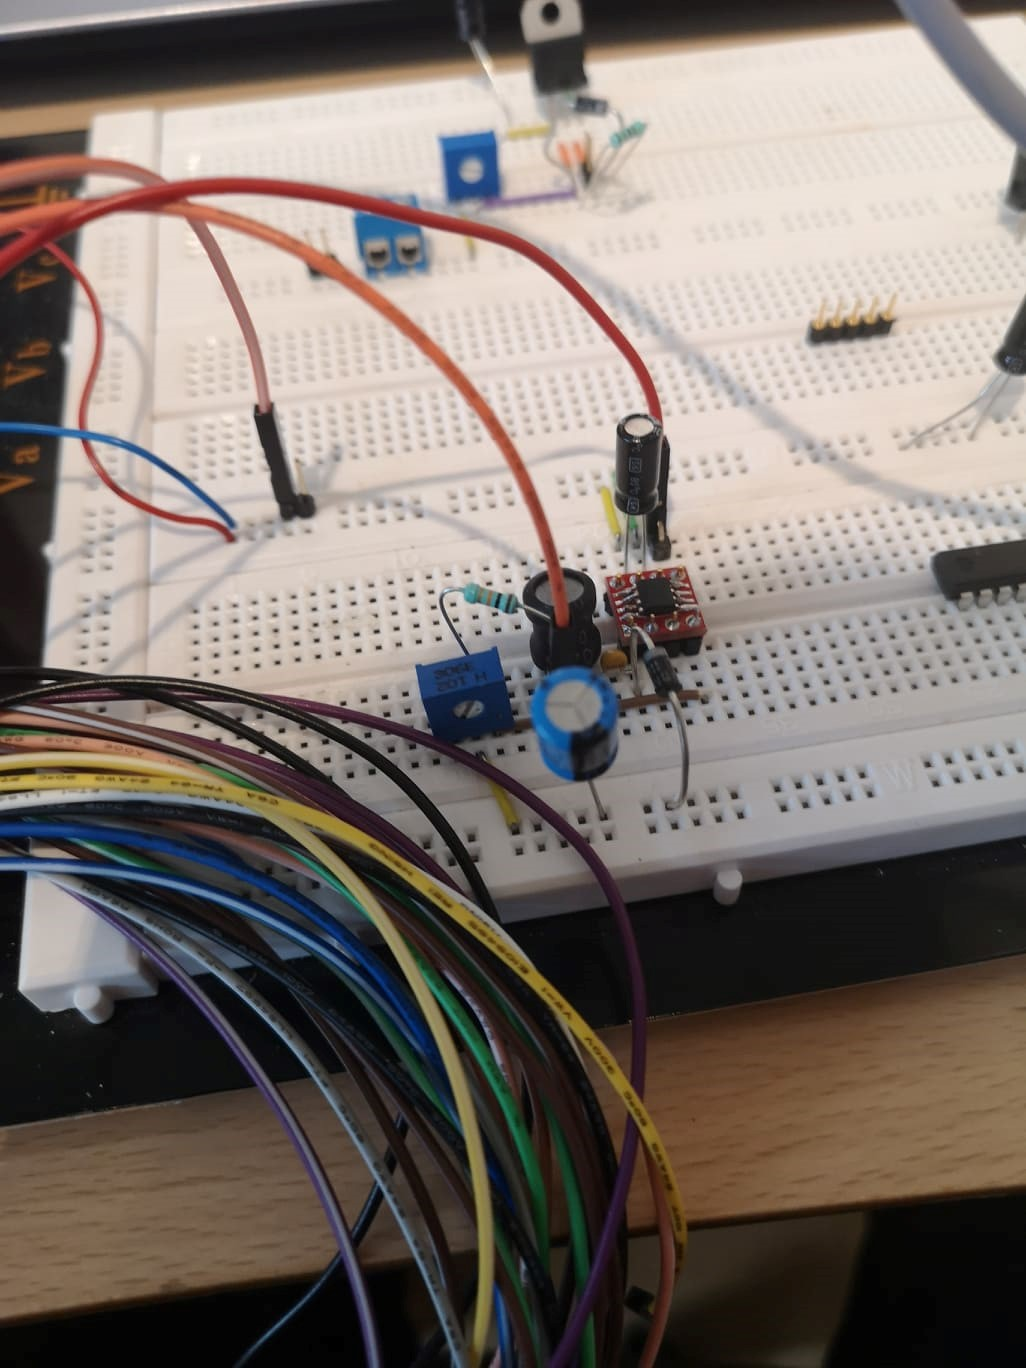
\includegraphics[width=0.3\textwidth]{bil6.jpg}
  \caption{}
  \label{fig:bil77}
\end{figure}

\textbf{Testresultater}\newline
Herunder ses resultater for testen. Først under almindelige omstændigheder.

\begin{figure}[h]
  \centering
  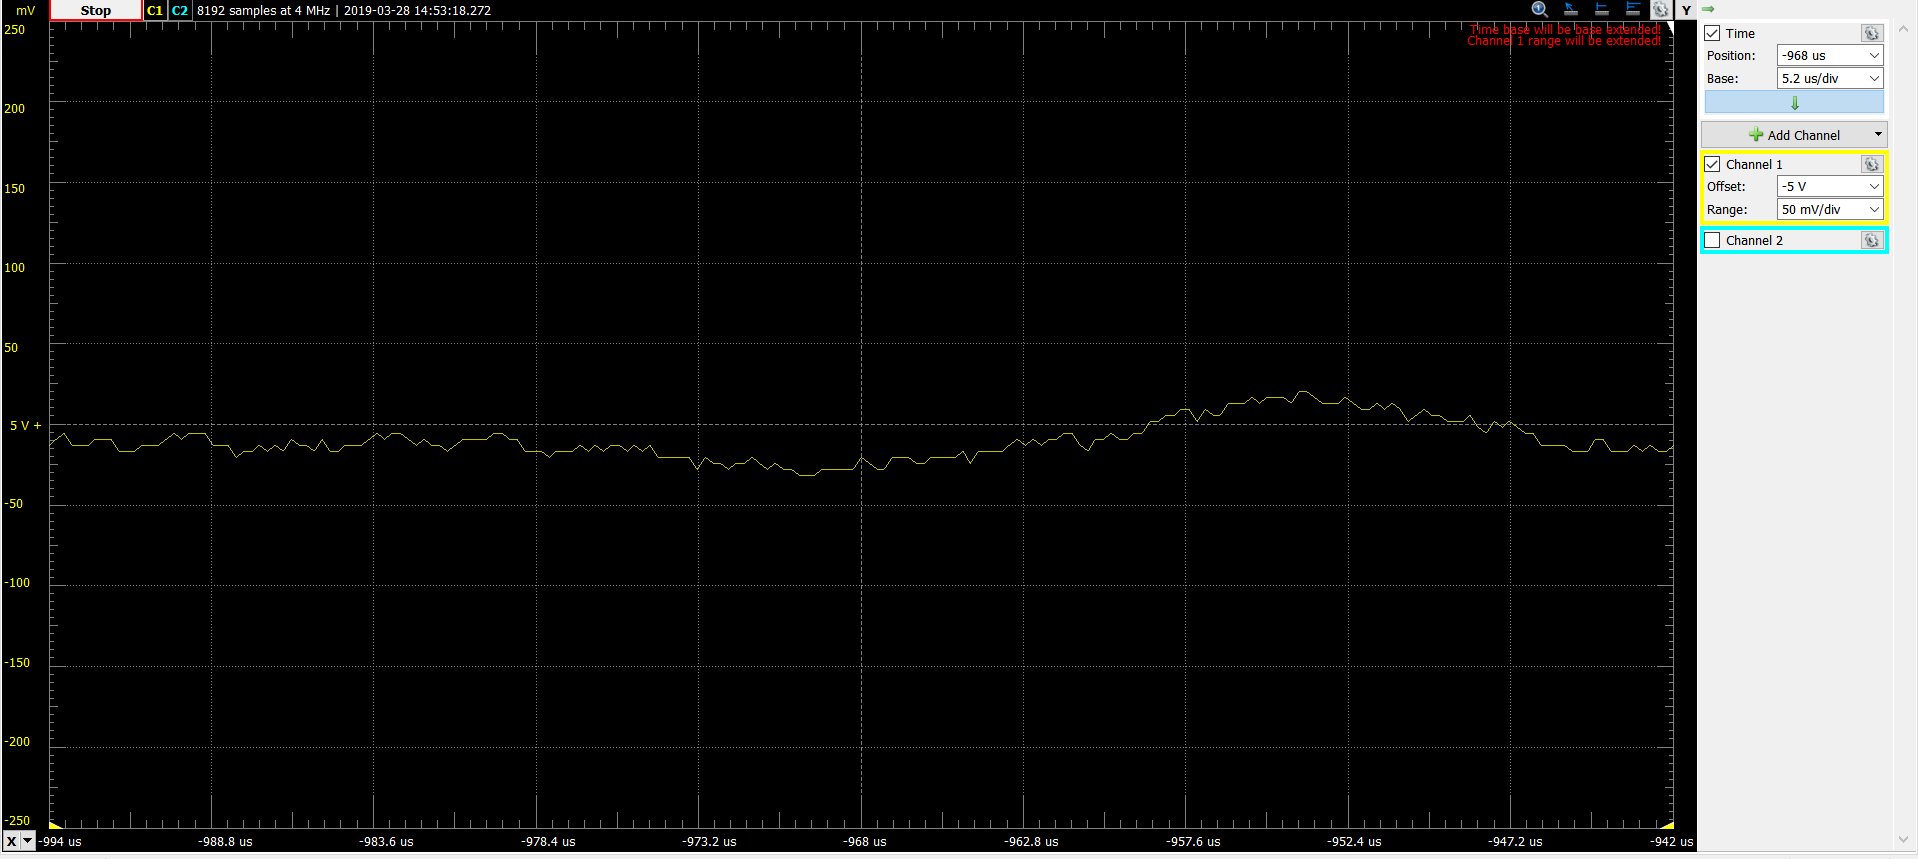
\includegraphics[width=0.3\textwidth]{bil7.png}
  \caption{}
  \label{fig:bil688}
\end{figure}
\clearpage
Som det ses, leveres en spænding omkring de 5 V. Denne spænding er acceptabel, om end vi ser en lille smule ripple. Denne kan skyldes den måde BUCK-konverteren virker på. Filteret der sidder efter konverteren, kan afvige en smule i praksis fra de teoretiske værdier. Det er dog stadig vigtigt at understrege, at dette output er acceptabelt. Strømmen måles til 1,3 A med loadmodstand.

Efter påvirkning af varme ændrede outputtet sig imidlertid ret dramatisk. Dette kan skyldes, at både dioden og TPS5410 er påvirkelige af varme, ligesom den induktive reaktans påvirkes i spolen. Her ses outputtet efter varmepåvirkningen har stået på i 30 sekunder. 
Som det ses af billedet, ændrer outputtet sig væsentligt! 
For at være sikker på, at komponenterne ikke var brændt af ved påvirkningen fra lighteren, køres en test cirka 15 minutter efter, hvor outputtet igen var standardiseret. 

\begin{figure}[h]
  \centering
  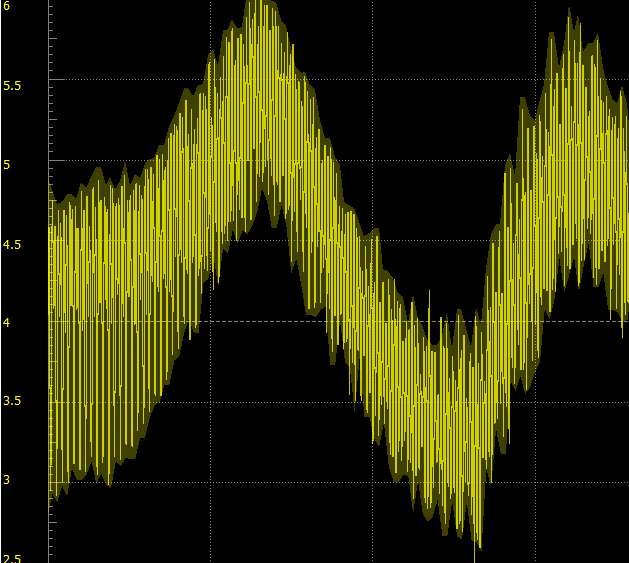
\includegraphics[width=0.3\textwidth]{bil8.png}
  \caption{}
  \label{fig:bil6}
\end{figure}

\subsection{Endeligt valg af system }
\label{sec:endeligt-valg-af}

På baggrund af netop gennemgåede test, vægtes systemerne mod hinanden på baggrund af det opstillede pointsystem. 
I første instans kan vi konkludere, at begge systemer er brugbare. De kan begge levere den ønskede strøm og spænding, og ripple på begge systemer er acceptabel. I skemaet herunder ses pointfordelingen imellem systemerne. 

\begin{table}[h]
  \centering
% BEGIN RECEIVE ORGTBL tabel3
\begin{tabular}{lrr}
\hline
\textbf{Komponent} & \textbf{TPS5410} & \textbf{LM317-T} \\
\hline
Varmepåvirkning & 0 & 2 \\
\hline
Billigste løsning & 0 & 2 \\
\hline
Minimal ripple & 0 & 1 \\
\hline
Minimal størrelse & 1 & 0 \\
\hline
Ialt & 1 & 5 \\
\hline
\end{tabular}
% END RECEIVE ORGTBL tabel3
  \caption{}
  \label{tab:komp3}
\end{table}
\begin{comment}
#+ORGTBL: SEND tabel3 orgtbl-to-latex :splice nil :skip 0
|-------------------+---------+---------|
| Komponent         | TPS5410 | LM317-T |
|-------------------+---------+---------|
| Varmepåvirkning   |       0 |       2 |
|-------------------+---------+---------|
| Billigste løsning |       0 |       2 |
|-------------------+---------+---------|
| Minimal ripple    |       0 |       1 |
|-------------------+---------+---------|
| Minimal størrelse |       1 |       0 |
|-------------------+---------+---------|
| Ialt              |       1 |       5 |
|-------------------+---------+---------|
\end{comment}


På baggrund af de opsatte kriterier vælges en spændingsregulator baseret på en LM317-T.

\clearpage
\subsection{Design - Endeligt system }
\label{sec:design-endel-syst}

Det endelige system har vi valgt at designe på PCB. Dette gøres fordi, at det er nemt at skrue ind i en vandtæt boks, så systemet ligger beskyttet og på denne måde møder vores sidste krav om at være vejrbestandigt. 
PCB-printet er designet i EAGLE, og er endt ud med designet som ses her ved siden af. Banerne er valgt til en tykkelse på 0,8 mm, hvilket sikre, at modstanden ikke bliver for høj taget strømstyrken i betragtning. Ulempen ved baner i den tykkelse er, at det øger risikoen for støj. Derfor har det også været vigtigt, at der ikke var nogle knæk på banerne, ligesom der er udlagt groundplane over resten af pladen. Dioden er ligeledes placeret et stykke fra IC’en, så de mest varmefølsomme komponenter ikke er placeret for tæt. Især da LM317-T også udstråler en anelse varme i drift. Der afsættes mellem 150 og 200 mW i LM317-T. 

\begin{figure}[h]
  \centering
  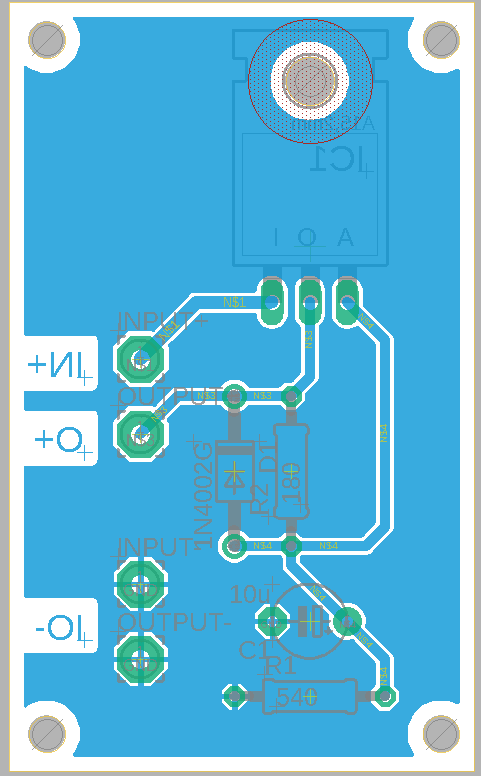
\includegraphics[width=0.3\textwidth]{bil9.png}
  \caption{}
  \label{fig:bil66}
\end{figure}
\clearpage
\section{PCB – Aktiv ensretter (Søren \& Thomas)}
\label{sec:pcb--aktiv}

I timebox 7 blev en nedskaleret version af kredsløbet til den aktive ensretter simuleret, bygget og testet på breadboard. Testen viste, at det valgte kredsløb fungerede efter hensigten, hvorfor der i denne timebox arbejdes videre med at designe et PCB print til den endelig version af ensretter-kredsløbet. PCB printet er designet med programmet, Eagle, og selve printet konstrueres af Jens Mortensen fra AU Herning ud fra .brd filen.

\subsection{Designovervejelser}
\label{sec:designovervejelser}

Den største udfordring i forhold til designet af PCB printet er umiddelbart den relative store strøm (op til 80 A peak), der i perioder vil komme til at løbe fra generatorens tre faser og ind i de tre MOSFETS, samt den lige så store strøm fra de øvrige tre MOSFETS til outputtet af kredsløbet. Der er med de konstruktionsmuligheder, som AU Herning stiller til rådighed, en begrænsning for maksimal bane bredde på printet, hvorfor det er besluttet at lave de førnævnte baner så korte og brede som mulige og så efterfølgende forstærke disse med evt. et stykke afklippet kobber, der bliver forbundet med de relevante MOSFETS. Banerne kan også yderligere forstærkes med et tykt lag tin efter konstruktionen af printet. Dette vil der blive taget hånd om, når komponenterne bliver loddet på printet (formentlig i timebox 9).

De øvrige baner på printet vil blive udført i en bredde på 0.6096 mm. 

Det er også diskuteret, hvordan de tre faser fra generatoren samt Vout og stel til outputtet skal kobles til printet, da de tilgængelige connectors i el-lab ikke umiddelbart kan håndtere den store strøm. For at være sikre på, at koblingen ikke bliver overophedet, er det besluttet at forbinde disse terminaler med en 3.5 mm bolt med passende spændeskiver og kabesko. Disse loddes sammen for at skabe en tilstrækkelig forbindelse med banerne.

\subsection{Eagle schematic}
\label{sec:eagle-schematic}

Den indledende del af designet af printet bestod af at lave et schematic tilsvarende kredsløbet benyttet til simuleringen og realiseringen i forrige timebox. Nedenstående figur viser et skærmbillede af det endelige schematic fra Eagle.

\begin{figure}[h]
  \centering
  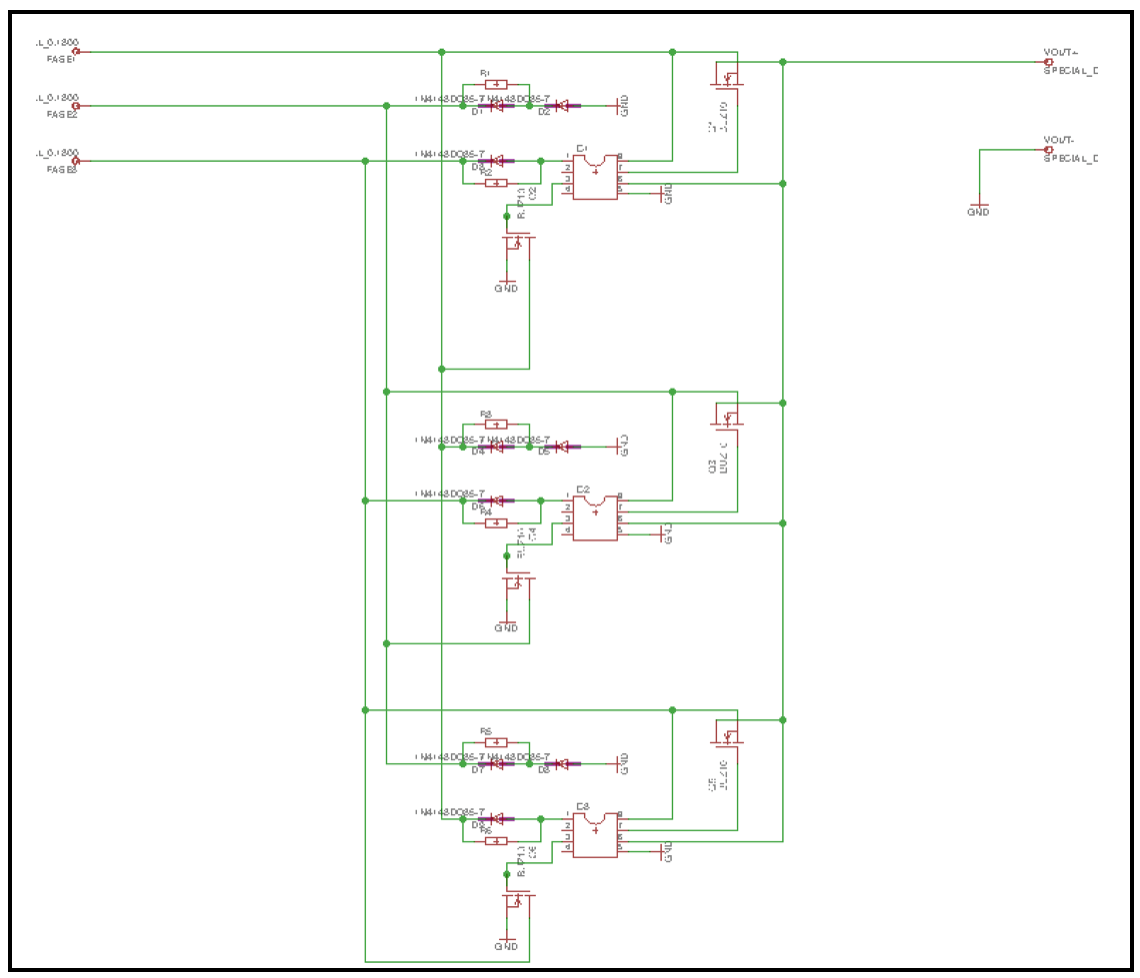
\includegraphics[width=0.3\textwidth]{dia3.png}
  \caption{Eagle schematic fra programmet, Eagle.}
  \label{fig:dia3}
\end{figure}
\clearpage
Næste del var at placere komponenter og trække baner i board delen af programmet, Eagle. Designet blev lavet på et tosidet print, således det var muligt at trække samtlige baner uden stort besvær. Nedenstående figurer viser et skærmbillede af top og bund laget fra designet. 

\begin{figure}[h]
  \centering
  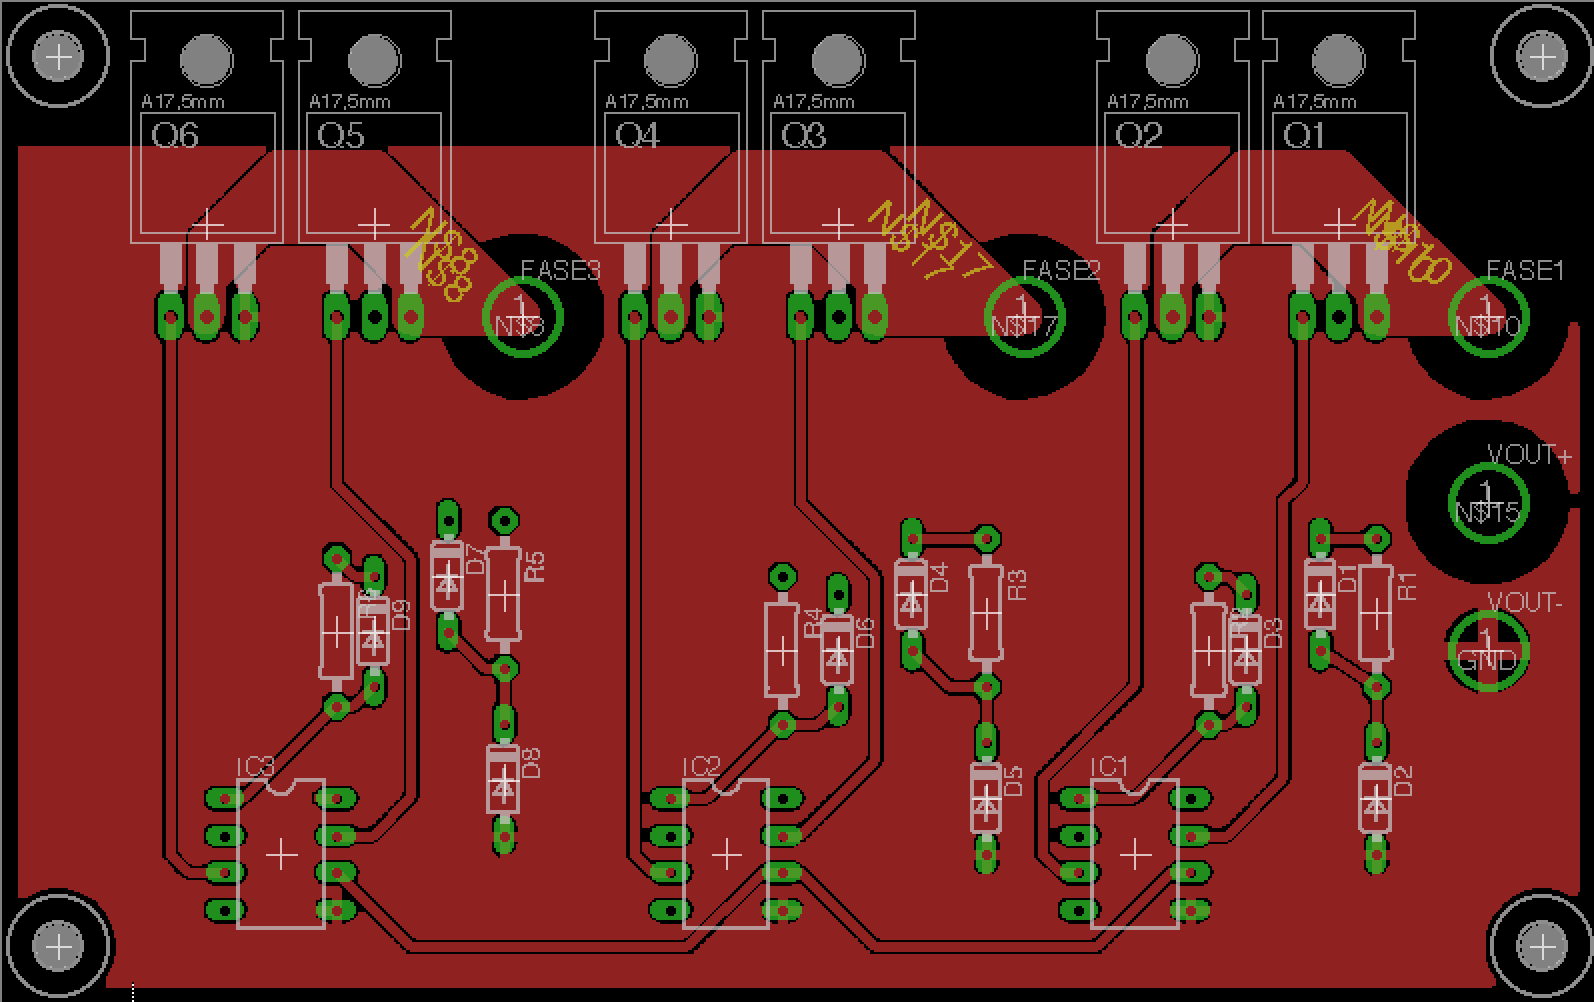
\includegraphics[width=0.4\textwidth]{dia4.png}
  \caption{Board designet fra Eagle, Top lag.}
  \label{fig:dia4}
\end{figure}

\begin{figure}[h]
  \centering
  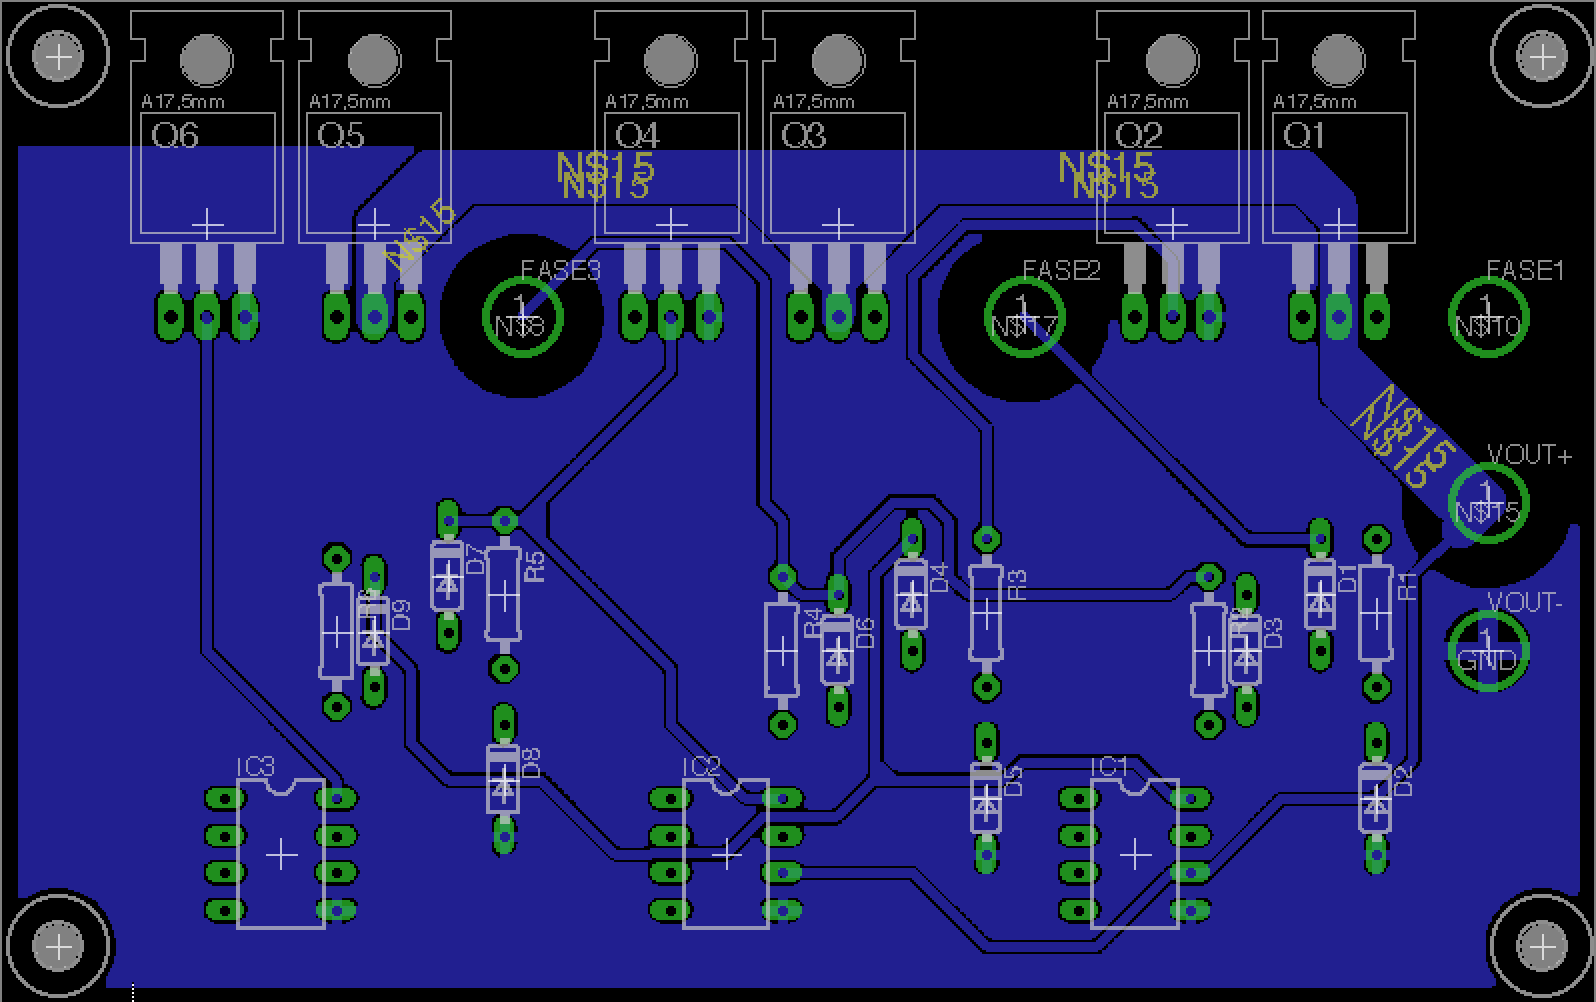
\includegraphics[width=0.4\textwidth]{dia5.png}
  \caption{Board designet fra Eagle, Bund lag.}
  \label{fig:dia5}
\end{figure}
\clearpage
På nedenstående figurer ses resultat af det færdigkonstruerede print.
\begin{figure}[h]
  \centering
  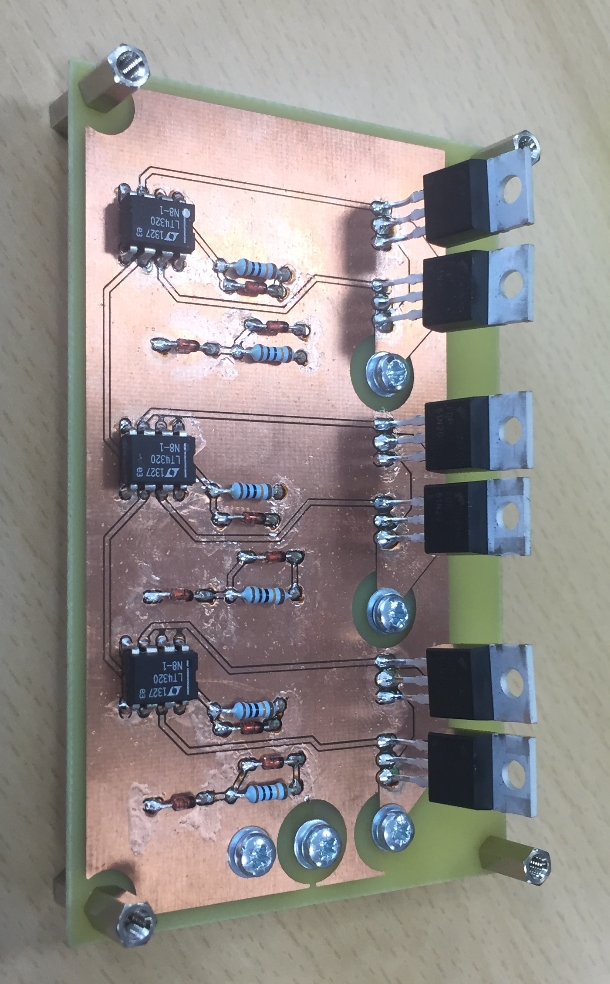
\includegraphics[width=0.25\textwidth]{dia6.png}
  \caption{PCB, Top lag.}
  \label{fig:dia6}
\end{figure}

\begin{figure}[h]
  \centering
  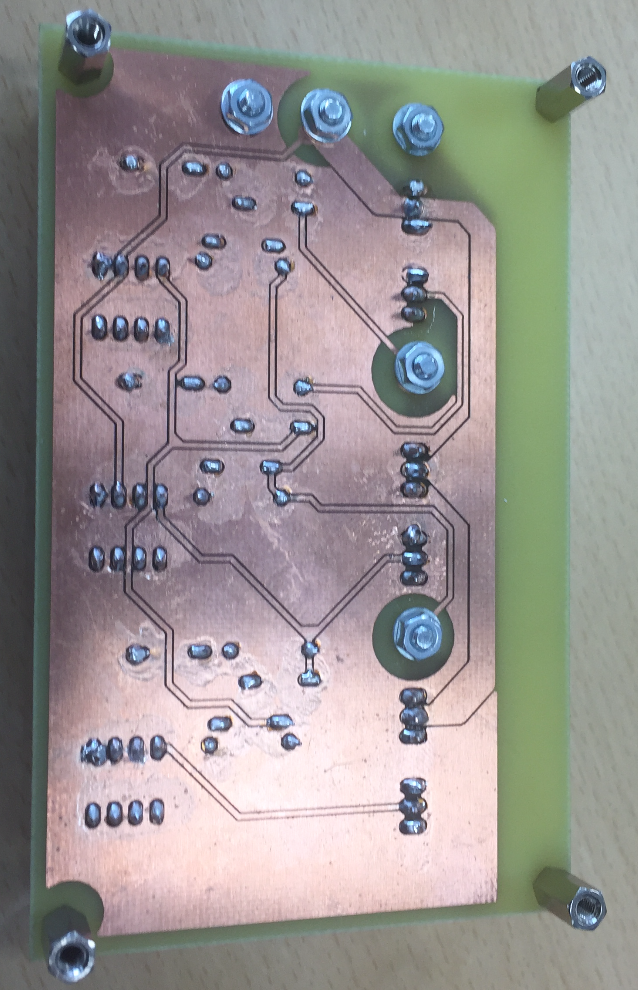
\includegraphics[width=0.25\textwidth]{diag7.png}
  \caption{PCB, Bund lag.}
  \label{fig:dia7}
\end{figure}
\clearpage
\section{Motorstyring (Simon)}
\label{sec:motorstyring-simon}

Der er tidligere blevet lavet målinger ved steprespons af forbrændingsmotor. Der er målinger af Hall-sensorens spænding, servomotoren der styre spjældets spænding, samt et tidsmål. Nedenfor ses et udsnit af de 50000 målinger:

\begin{table}[h]
  \centering
% BEGIN RECEIVE ORGTBL tabel4
\begin{tabular}{r|r|r}
\hline
\textbf{second} & \textbf{Volt} & \textbf{Volt1} \\
\hline
-1 & 0.215206000000000 & 4.98492460000000 \\
-0.999900000000000 & 0.215206000000000 & 4.90452260000000 \\
-0.999800000000000 & 0.134804000000000 & 4.90452260000000 \\
-0.999700000000000 & 0.215206000000000 & 4.98492460000000 \\
-0.999600000000000 & 0.215206000000000 & 4.90452260000000 \\
-0.999500000000000 & 0.215206000000000 & 4.90452260000000 \\
-0.999400000000000 & 0.215206000000000 & 4.90452260000000 \\
-0.999300000000000 & 0.215206000000000 & 4.82412060000000 \\
-0.999200000000000 & 0.215206000000000 & 4.90452260000000 \\
\hline
\end{tabular}
% END RECEIVE ORGTBL tabel4
  \caption{}
  \label{tab:komp3}
\end{table}
\begin{comment}
#+ORGTBL: SEND tabel4 orgtbl-to-latex :splice nil :skip 0
|--------------------+-------------------+------------------|
|             second |              Volt |            Volt1 |
|--------------------+-------------------+------------------|
|                 -1 | 0.215206000000000 | 4.98492460000000 |
| -0.999900000000000 | 0.215206000000000 | 4.90452260000000 |
| -0.999800000000000 | 0.134804000000000 | 4.90452260000000 |
| -0.999700000000000 | 0.215206000000000 | 4.98492460000000 |
| -0.999600000000000 | 0.215206000000000 | 4.90452260000000 |
| -0.999500000000000 | 0.215206000000000 | 4.90452260000000 |
| -0.999400000000000 | 0.215206000000000 | 4.90452260000000 |
| -0.999300000000000 | 0.215206000000000 | 4.82412060000000 |
| -0.999200000000000 | 0.215206000000000 | 4.90452260000000 |
|--------------------+-------------------+------------------|
\end{comment}

Der fokuseres spændingsmålet Volt1 fra Hall-sensoren.
Når data plottes for et kort tidsrum ses støj omkring 5 volt

\begin{figure}[h]
  \centering
  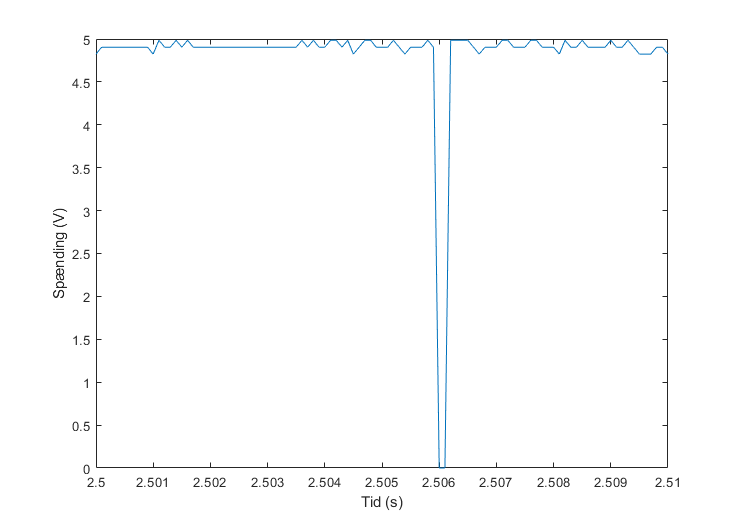
\includegraphics[width=0.6\textwidth]{mo1.png}
  \caption{}
  \label{fig:mo1}
\end{figure}

Data processeres nu med følgende Matlab-script:
\begin{lstlisting}[language=Matlab]
close all
data = stepdata5;
t = data.second;
v = data.Volt1;
border1 = 4.5;
border2 = 0.1;
v2 = data.Volt;
b = 0;
stop = 0;
tp = [];
tpt = [];
vpt0 = [];
i = 1;
nyv = [];
while (i <= length(t))
    if (v(i)>border1)
        vn = 5;
    else
        vn = 0;
    end
    nyv = [nyv vn];
    i = i + 1;
end
i = 1;


while (i < length(t))
    if ((nyv(i+1)>border1 & nyv(i)<border2) & b == 0)
        t1 = t(i+1);
        stop = 1;
        b = 1;
    end
    i = i + 1;
    vpt0 = [vpt0 0];
    while (stop ~= 2 & b == 1 & i < length(t))
        if (stop == 1)
            while (stop ~= 2 & i < length(t))
                if (nyv(i+1)>border1 & nyv(i)<border2)
                    t2 = t(i+1);
                    stop = 2;
                end
                i = i + 1;
                vpt0 = [vpt0 0];
            end
        end
        if (stop == 2)
            period = t2-t1;
            tpt = [tpt t2];
            vpt0(i) = nyv(i);
            tp = [tp period];
            t1 = t2;
            stop = 1;
        end
    end
end  
\end{lstlisting}
\clearpage
I scriptet fortolkes spænding over 4,5 V som 5 V. Markering af periodegrænser ved 5 Volt kan ses her (de røde prikker øverst):

\begin{figure}[h]
  \centering
  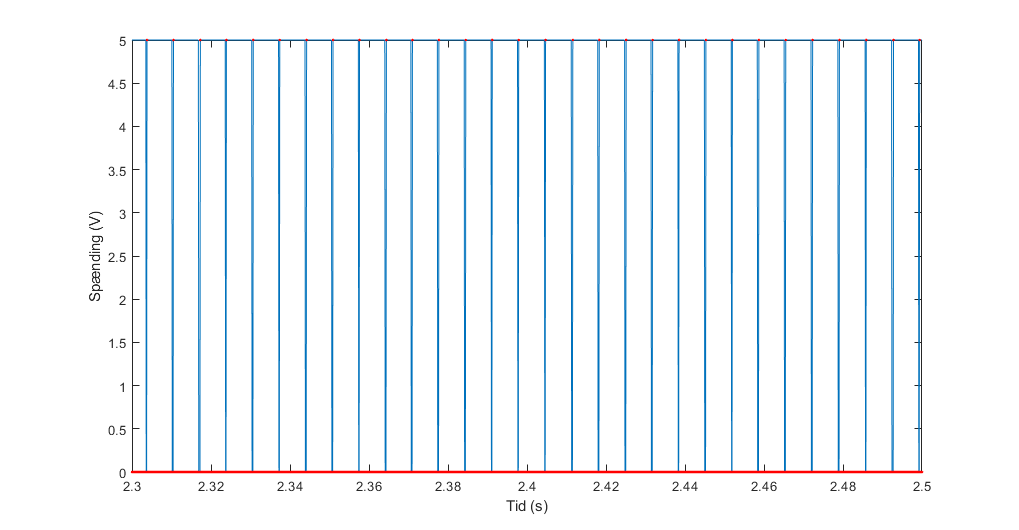
\includegraphics[width=0.6\textwidth]{mo2.png}
  \caption{}
  \label{fig:mo2}
\end{figure}

Herudover udregnes tiden for hver omdrejningsperiode og gemmes i vektoren ”tp”.
Ved plot at tp udregnet som rpm og plottet overfor tid fås:

\begin{figure}[h]
  \centering
  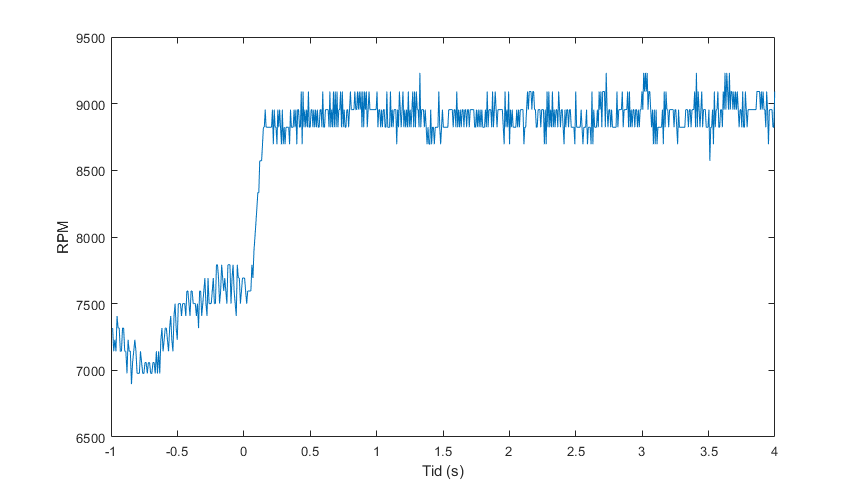
\includegraphics[width=0.6\textwidth]{mo3.png}
  \caption{}
  \label{fig:mo3}
\end{figure}
\clearpage
Scopet der har målt data gemmer også data op til stepresponset. Stepresponset ses ved tiden 0.
Ved at applicere et midlingsfilter på 200 fås et indtryk af et steady-state niveau ved 8900, med start fra 7600, dvs 1300. 

\begin{figure}[h]
  \centering
  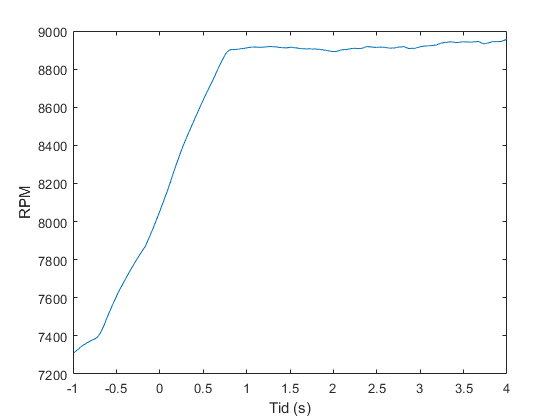
\includegraphics[width=0.5\textwidth]{mo4.png}
  \caption{}
  \label{fig:mo4}
\end{figure}

Ved at applicere et midlingsfilter på 10 fås et indtryk af en 1. grads overføringsfunktion.

\begin{figure}[h]
  \centering
  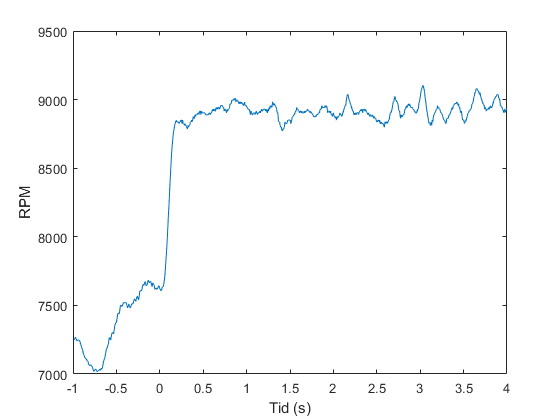
\includegraphics[width=0.5\textwidth]{mo5.png}
  \caption{}
  \label{fig:mo5}
\end{figure}

Det måles at steady-state er opnået ved 0,19 sekunder. Dvs. $0.81 = 5\tau \Leftrightarrow \frac{0,19}{5}=\tau=0,04$.

Hermed kan overføringsfunktionen sættes som
\begin{equation}
  \label{eq:1}
G(s) = \frac{1300}{0,04s+1}  
\end{equation}
\clearpage
\section{Deployment (Alle)}
\label{sec:deployment}
I denne timebox deployes valg af LM317-T til og design af spændingsregulator. Herudover deployes PCB design af den aktive ensretter og fund af overføringsfunktion for motorstyring.
Hermed godkender kunderne, Morten Oppbrud Jakobsen og Jan Møller Nielsen, ovenstående i timebox 8.

Mandag den 13/5-2019

\begin{minipage}{.5\textwidth}
  \begin{center}
    \vspace{1.4cm}
    \rule{0.8\textwidth}{0.1pt}\\
    \small{Morten Opprud Jakobsen\\%\vspace{0.1cm}\textit{Projektansvarlig læge}
    }
  \end{center}
\end{minipage}%
\begin{minipage}{0.5\textwidth}
  \begin{center}
    \vspace{1.4cm}
    \rule{0.8\textwidth}{0.1pt}\\
    \small{Jan Møller Nielsen\\%\vspace{0.1cm}\textit{Forskningsansvarlig overlæge}
    }
  \end{center}
\end{minipage}

% \printbibliography
\end{document}